\section{Conclusions \& Improvements}
Looking at the results, there were a few big issues. 
From the results we found that we are missing a couple of features of the application, and the majority of issues are design related problems.

The most commonly reported issues on the feature side were related to how the user cannot disconnect and connect to another server and that there should be an error message signaling whether the address is wrong or if the current address does not exist. There is no distinction between connecting as admin and connecting as user. The rest of the data refers to minor inconveniences such as the size of editing inputs and changing other elements of the board/cards.

On the design side the most common problems were the drag and drop functionality that seemed to be unclear for the users, and there were also some problems with our colour scheme of choice that confused the users.The lack of colour contrast could make it hard to distinguish the different elements in the window and the colour coding was not consistent for all the elements.
The rest of the feedback includes emitting error messages or warnings when things with the same names are added, and more general text conventions like text size/positioning and button placement and grouping in the page. The most important functionality that will be implemented is to make sure the client can successfully connect and disconnect to different servers including visible errors and warnings for better user experience. 

\subsection{Improvements}
Below, you can find the improvements we're performing. Not all problems have been improved on, since 4 feature problems were not a requirement for our prototype and 11 design problems were a personal preference of the expert or the expert misunderstood some drawing in the prototype. For instance, a few didn't find it clear that you could move cards between lists. This was the intended behaviour but we only showed moving cards within a list itself.

\subsubsection{Features}
\begin{itemize}
    \item Disconnect
    \item Server address incorrect / error
\end{itemize}

\subsubsection{Design}
\begin{itemize}
    \item Buttons in pop up windows do not mix well with background 
    \item Standard button format
    \item Default new list/card names in add windows, you can't add the card if it doesn't have a name
\end{itemize}

\subsection{The new and improved GUI}
We've redesigned and/or improved the following interfaces:

\subsubsection{The connect window}
The connect window now has a completely new UI design, along with space for an error message.

\begin{figure}
    \centering
    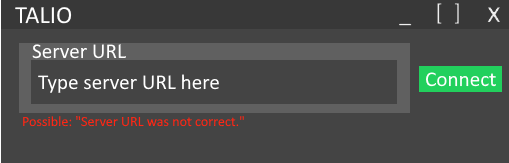
\includegraphics{images/TALIOconnect.png}
    \caption{New connect window with a possible error message}
    \label{fig:Connect Window}
\end{figure}

\subsubsection{The board overview}
The board overview now has a disconnect button in the top left. Instead of boardName, it now has TALIO in the top. As our application cannot yet have multiple boards. 

\begin{figure}
    \centering
    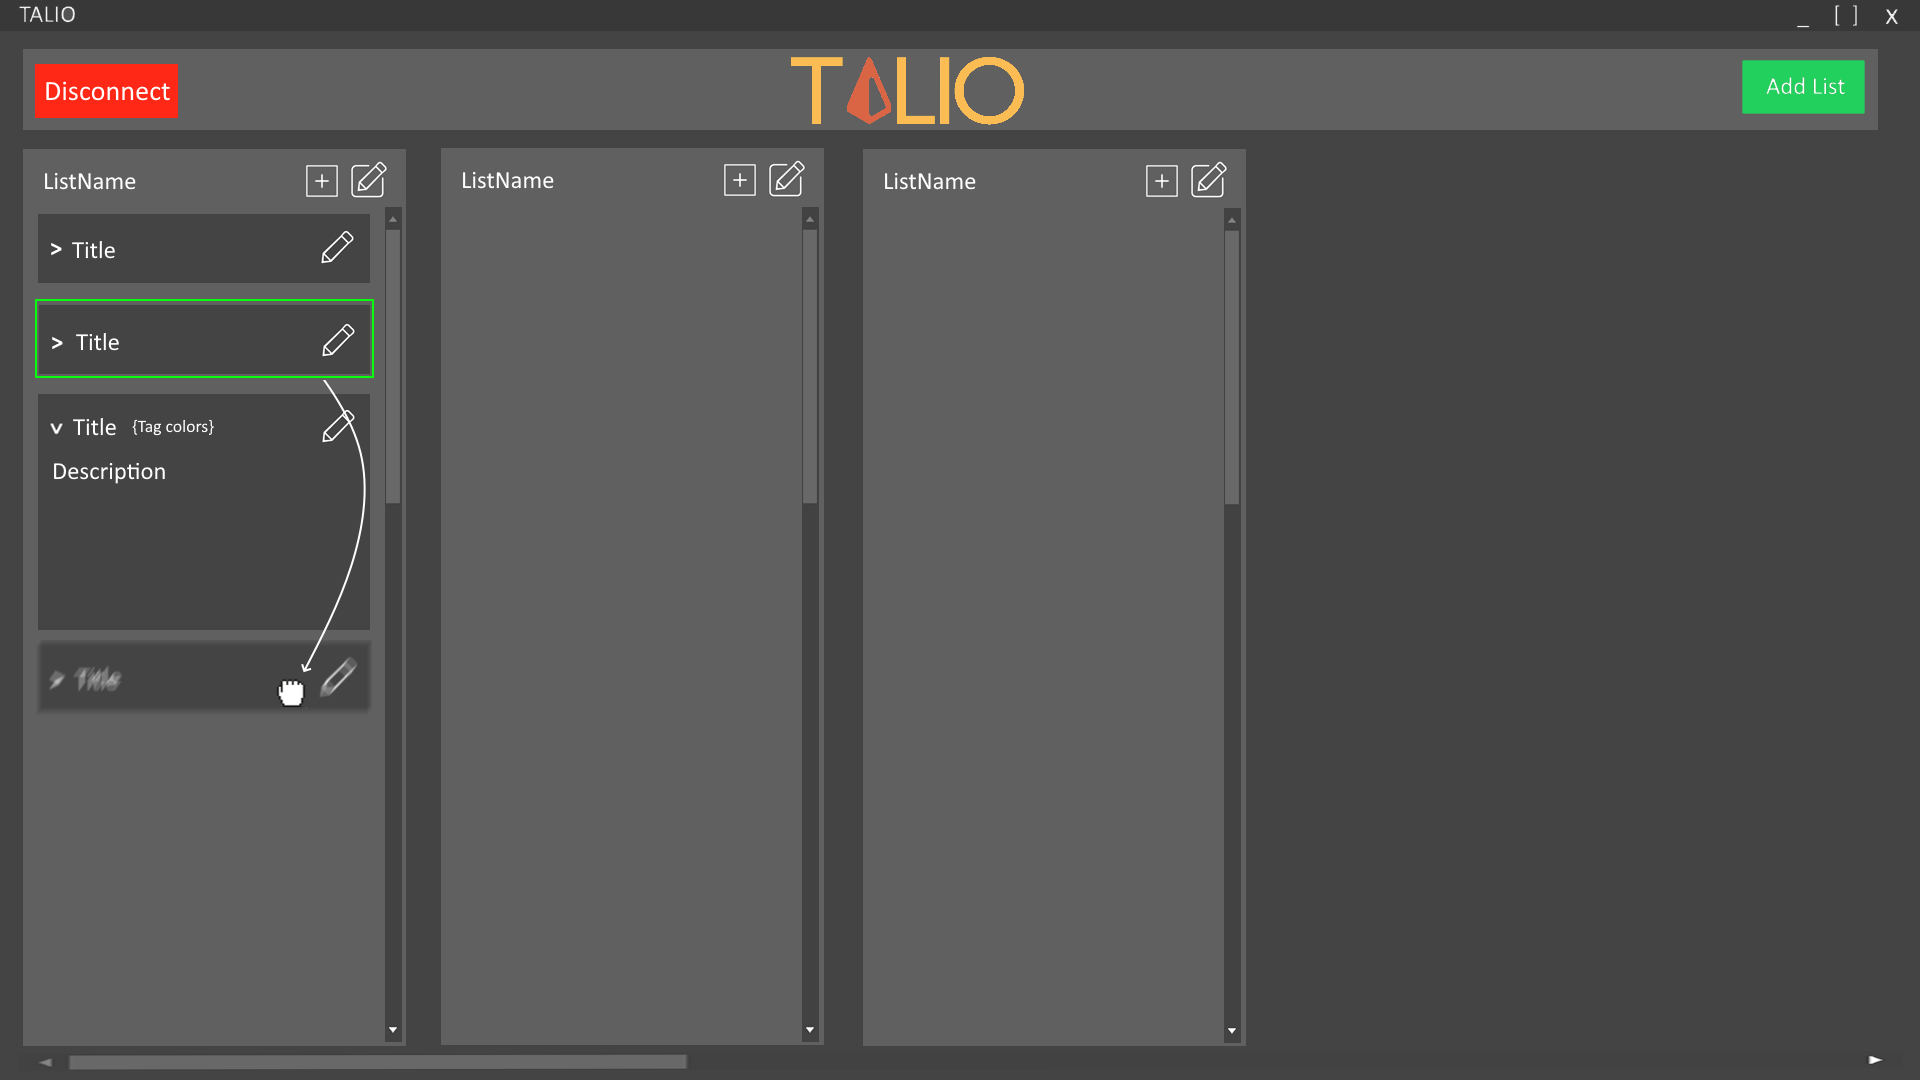
\includegraphics[scale=0.4]{images/UI design Board.png}
    \caption{Board overview with new title and a disconnect button}
    \label{fig:Board Overview}
\end{figure}



\subsubsection{The add/edit list/card windows}
These now have a standard button design, similar to the board overview. The colors have also been adjusted.
The add card/list windows now have sample text in the title area. 

\begin{figure}
    \centering
    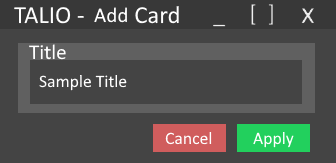
\includegraphics{images/UI design addCard.png}
    \caption{Add card window with new button and sample title}
    \label{fig:addCardWindow}
\end{figure}
\begin{figure}
    \centering
    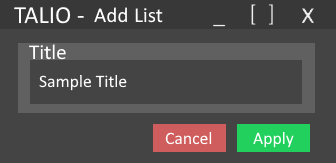
\includegraphics{images/UI design addList.png}
    \caption{Add list window with new button and sample title}
    \label{fig:addListWindow}
\end{figure}
\begin{figure}
    \centering
    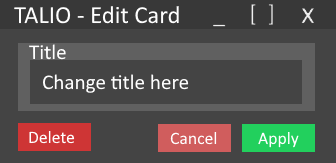
\includegraphics{images/UI design editCard.png}
    \caption{Edit card window with new buttons}
    \label{fig:editCardWindow}
\end{figure}
\begin{figure}
    \centering
    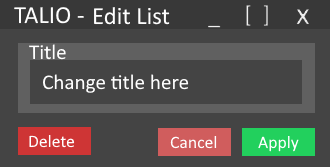
\includegraphics{images/UI design editList.png}
    \caption{Edit list window with new buttons}
    \label{fig:editListwindow}
\end{figure}